\chapter{Grid Search}
\label{ch4}
This chapter walks through the methodology used to select the best model and parameters to forecast 4 hours of $C_{n}^{2}$ given prior environmental measurements, then the statistical analysis performed as a justification for the model selection.

\section{Methodology}
Given a problem to model with machine learning there are model hyperparameters to adjust in infinitely many combinations, each of which can impact model performance. Just a few examples of these hyperparameters are the optimization algorithm, the learning rate of the optimization algorithm, the number of layers in a model architecture and the number of nodes per layer. Given the many combinations of a model's hyperparameters, a careful method to determine the best combination must be employed. The definition of the ``best" model is the model which results in the best performance when applied to the validation dataset, a subset of the entire dataset specifically held from training for hyperparameter tuning. By holding back the validation dataset, an unbiased optimization of the hyperparemeters can be performed, then those parameters are used in the model applied to the test dataset for an unbiased evaluation of the final model.

There are many methods of hyperparameter optimization, but common methods are grid search and random search. Grid search, or a parameter sweep, is an exhaustive search through manually specified hyperparameters. If iterating over only one hyperparameter, for example three different learning rates, a model is trained with the first learning rate and it's performance on the validation dataset is recorded, then the model is trained again in the same fashion but with the second learning rate and the performance on the validation dataset is recorded, and finally this is done again for the third learning rate. The performance of the models with the three learning rates are compared and the best learning rate is the learning rate used by the model that performed best. This method can quickly explode in computation time as the number of hyperparameters to iterate increases. For example, iterating over two hyperparameters of three values each results in nine combinations of hyperparameters. The number of combinations is defined as the multiple of the number of values across each hyperparameter, so if there are five hyperparameters with 1, 2, 3, 4, and 5 values, then the total number of combinations is $1 \times 2 \times 3 \times 4 \times 5 = 120$ combinations.

The other common method, the random search, replaces the exhaustive grid search by randomly selecting hyperparameters within defined bounds. An algorithm randomly selects the hyperparameters and models are trained with the different combinations then applied to the validation dataset to evaluate performance. The hyperparameters associated with best performing model are the best hyperparameters. A benefit of the random search is the selection of parameter combinations that might not be defined in a grid search.

In this work the grid search is employed because prior knowledge of hyperparameters is unknown, thus the exhaustive grid search is necessary to explore a wide range of combinations. This grid search iterates over five parameters. The outermost parameter is the four fundamental architectures: MLP, simple RNN, GRU, and LSTM. The MLP is a common machine learning architecture and serves as a baseline. The simple RNN, GRU, and LSTM are variants of the general RNN and are searched to find if a specific variant is better or worse than the others when applied to this problem. The next parameter is the input sequence variables used by the model. From Section \ref{sec:wx_seq_hist}, the available input sequence features (variables) are prior temperature, pressure, relative humidity, wind speed, solar irradiance, and $C_{n}^{2}$ measurements. The ``input sequence features" parameter iterates over which features (variables) to train the model. Since there are six available features, and each feature can only be used or not used, there are $2^6 = 64$ total combinations. However, a threshold is set to train on a minimum of four features which reduces the total number of input feature combinations to 22. This threshold is set to discourage the model from memorizing one or two features, and for a significant reduction in computation time. The third search parameter is the input sequence length. Independent of the input features (variables), in a single sequence/forecast the amount of information available to the model is dependent on the time-length of the input sequence. Whether the model performs best with only 4 hours of input data or 16 hours of input data is highly relevant information. Thus, four lengths of the input sequence are searched: 4, 8, 12, and 16 hours. These lengths are chosen to be $1\times$, $2\times$, $3\times$, and $4\times$ the 4 hour forecast length. Note that the train, validation, and test datasets are carefully formatted so the same forecasts are trained, validated, and tested regardless of the input sequence length. This avoids an instance where a 4-hour input sequence might exist for a particular forecast but a 16 hour input sequence is not available due to missing data. The fourth parameter searched is the number of hidden layers in each architecture: 1 or 2. The fifth and final searched parameter is the number of hidden nodes per hidden layer: 10 through 50 in steps of 10. The final two parameters essentially search over the number of parameters in the model with some variation in the interaction of those parameters. Each fundamental architecture in total iterates over $22 \times 4 \times 2 \times 5 = 880$ combinations of parameters. Due to the stochastic nature of model training, a single model could perform significantly different than another model trained with the same parameters, thus a total of 10 models are trained per combination per fundamental architecture to ensure the stability of results. In this search a total of $880 \times 4 \times 10 = 35,200$ models are trained.

For each model trained in the grid search the following parameters are fixed: mini-batch size, optimization algorithm, initial learning rate, learning rate decay (step and decay factor), and weight decay. The mini-batch size, the number of training examples used per model parameter update, is set to 32 yielding a total of 30 parameter updates (933/32) per epoch (iteration through the entire dataset). The optimization algorithm is AdamW, one of the most popular optimization algorithms used today (\textcolor{blue}{Go in depth about the algorithm here, or reference the background section? Reference paper on Adam, paper on correct implementation of regularization term, AdamW, and pytorch implementation}). The initial learning rate is 0.01 and decays by a factor of 10 every 10 epochs. This results in learning rates 0.01, 0.001, 1e-4, 1e-5, and 1e-6 from epochs 1 - 10, 11 - 20, 21 - 30, 31 - 40, and 41 - 50, respectively. The high initial learning rate is to ensure suitably-high gradients are back-propagated through the model to allow each model 10 epochs (300 total parameter updates) to escape any local minima. This training method consistently leads to a strong model convergence in only a few seconds. The weight decay is a regularization technique applied to the optimization algorithm and is 0.001 \textcolor{blue}{there is no reason why I chose this specific value, 1e-3; I just wanted to employ a bit of regularization to avoid overfitting}.

\section{Results}
The analyses of the grid search are performed independently on each architecture. From the four grid searches, four 2d-arrays of RMSE loss scores, the performance metric between validation truth and output $log_{10}(C_{n}^{2})$, are recorded for analysis. The 2d-arrays are of shape $880 \times 10$ for 880 parameter combinations and 10 models each. From these four 2d arrays, the average and standard deviation (degrees of freedom = $N - 1$) of the RMSE scores are calculated per parameter combination yielding four arrays of 880 averages and standard deviations of RMSE scores. The standard error, or the standard deviation of the mean, is calculated by dividing the standard deviation by the square root of the number of samples, 10 in this case \textcolor{blue}{add equations here!}. From these statistics the best model is determined and significance quantified.

The four arrays of average RMSE scores are sorted from best to worst and the sort indices are applied to the array of grid search parameters. From these sorted arrays the best model and its parameters are extracted. Figure \ref{fig:grid_search_results} illustrates the validation average $log_{10}(C_{n}^{2})$ RMSE loss as a function of the sorted index. Figure \ref{fig:grid_search_results_a} plots all 880 sorted scores for each fundamental architecture. Figure \ref{fig:grid_search_results_b} plots only the first ten to focus on the best performers. In each plot MLP is drawn in blue, RNN in orange, GRU in green, and LSTM in red. The curves in each figure are monotonically increasing because the sorted losses are plotted. Figure \ref{fig:grid_search_results_b} additionally plots the standard deviation of the mean, or the standard error, from Equation \textbf{REFERENCE EQUATION HERE}.
\begin{figure}[h!]
	\centering
	\subfloat[Full set of iterations\label{fig:grid_search_results_a}]{
		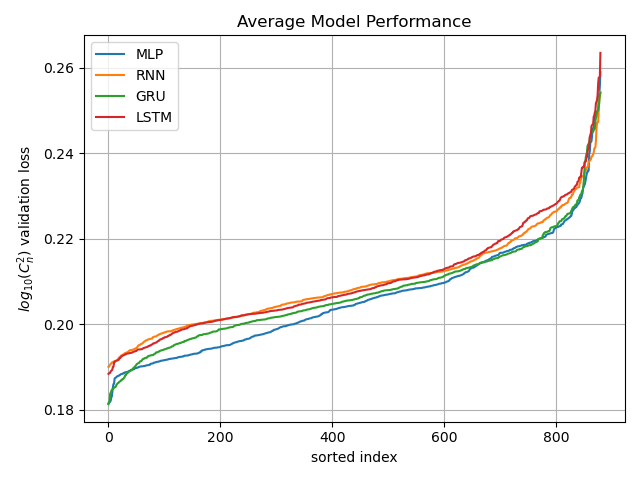
\includegraphics[width=0.49\textwidth]{average_model_performance_wide.png}
	}
	\subfloat[Top 10 iterations\label{fig:grid_search_results_b}]{
		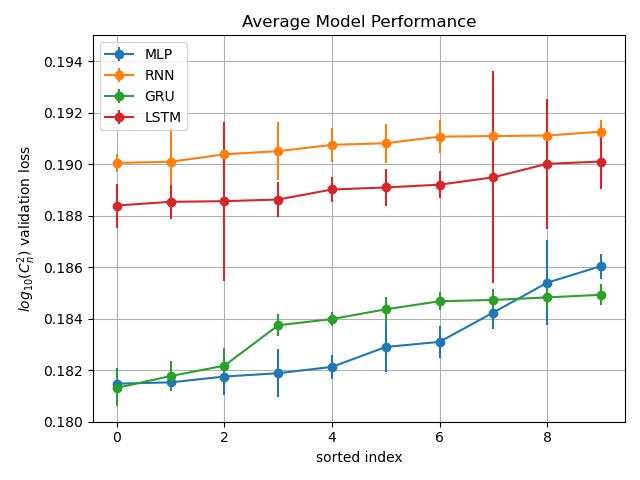
\includegraphics[width=0.49\textwidth]{average_model_performance_narrow.png}
	}
	\hfill
	\caption{Grid search results.}
	\label{fig:grid_search_results}
\end{figure}
The curves in Figure \ref{fig:grid_search_results_a} generally indicate that over the grid search space the MLP dominates the ensemble of RNN architectures. The general shape of the sorted loss curves are highly correlated from architecture to architecture. It's also interesting to note that the slope of the loss curves are very steady from sorted index 100 through 800. On the worse side of the sorted indices, beyond index 800, the loss curves exponentially increase. Likewise on the better side of the sorted indices, from 0 to 100, the loss curves also exponentially increase. Throughout the sorted indices, but most importantly at the beginning (left) of the sorted indices, the MLP (blue) and GRU (green) architectures perform better by a large margin compared with the simple RNN (orange) and LSTM (red) architectures. This is further shown in Figure \ref{fig:grid_search_results_b} which illustrates the first ten sorted indices of Figure \ref{fig:grid_search_results_a}. The loss curves illustrate that on average the best ten models of the simple RNN is the worst of the four architectures and the best ten models of the LSTM models are a scale factor better. Further, the best ten MLP and GRU models are very similar, even crossing over each other twice. At first glance of Figure \ref{fig:grid_search_results_b} it appears the MLP is generally the best model, but upon closer inspection the best GRU is very slightly better than the best MLP. Specifically, the validation average $log_{10}(C_{n}^{2})$ is 0.181476 and 0.181316 for the best MLP and GRU models, respectively.

\textcolor{blue}{Describe student's t-test and the plot in Figure \ref{fig:students_t-test}}.
\begin{figure}[h!]
	\centering
	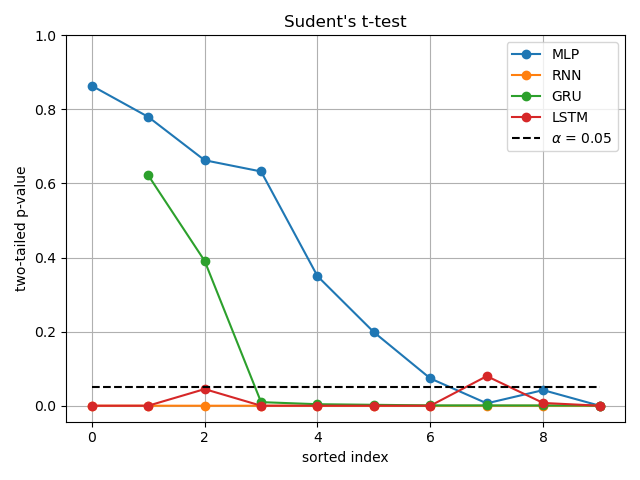
\includegraphics[width=0.7\textwidth]
	{students_t-test.png}
	\hfill
	\caption{Grid search results.}
	\label{fig:students_t-test}
\end{figure}
\textcolor{blue}{Describe Figure \ref{fig:variable_sets_analysis} and how it is a variable sensitivity analysis.}
\begin{figure}[h!]
	\centering
	\subfloat[Best 10\%\label{fig:variable_sets_analysis_a}]{
		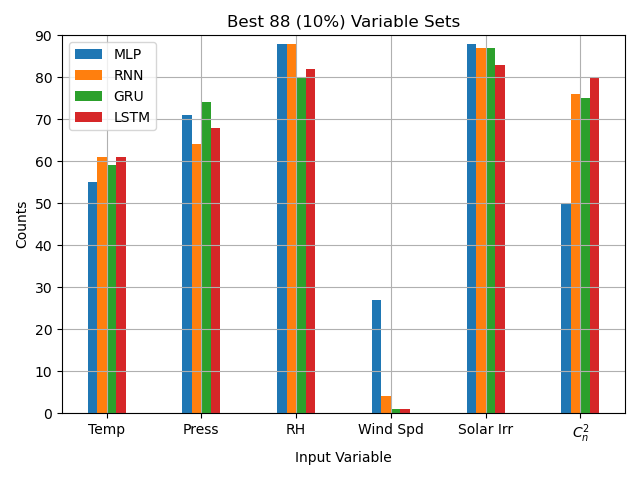
\includegraphics[width=0.49\textwidth]{bar_variable_sets_best.png}
	}
	\subfloat[Worst 10\%\label{fig:variable_sets_analysis_b}]{
		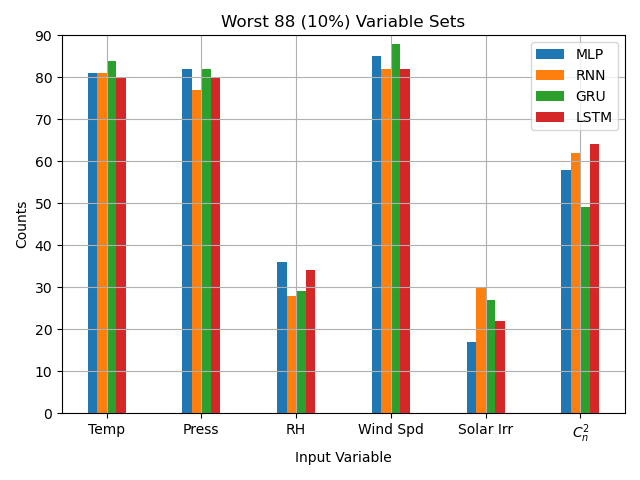
\includegraphics[width=0.49\textwidth]{bar_variable_sets_worst.png}
	}
	\hfill
	\caption{Best 10\% and worst 10\% variable sets.}
	\label{fig:variable_sets_analysis}
\end{figure}
\textcolor{blue}{Write reasons for picking the best GRU model: best average score, standard error is similar to next best MLP model, shorter data requirement, no real reason to pick MLP}.